% !TEX root=/home/tavant/these/manuscript/src/manuscript.tex




\chapter{Polytropic sheath model in the presence of electron emission}
\label{ch-4}

\begin{Chabstract}
  
%e modify the polytropic sheath model with secondary electron emission
We add to the non-isothermal sheath model developed in \cref{ch-3} the secondary electron emission.
using the \ac{PIC} simulations, we observe that the polytropic index is almost constant when varying the cross-over energy $\crover$.
The predictions of the polytropic sheath model are compared to the \ac{PIC} simulations results presented in \cref{ch-2}.
The modified sheath model is included in a \ac{1D} fluid model.
\end{Chabstract}

{\bf IV. Polytrotic sheath model with SEE} 20 pages
\begin{zzz}
  This chapter goes beyond the actual modified sheath model in order to add SEEs.
  This require some time to develop before writting !

  5.1 Kinetic effects of the SEE on the EVDFs  4 pages

  5.2 SEE effects on the Fluid model  5 pages

  5.3 Validation against the Parametric 2D PIC simulation results. 2 pages
  
  5.4 1D fluid model with modified wall model. 4 pages
  
  5.4Bis Global model (Vivien's) with modified wall model. 4 pages
\end{zzz}

\minitoc
% 
% What is complicated here is the definition of the electron temperature, that include both primary and secondary electrons.
% Should we
% \begin{itemize}
%   \item Use a 2 fluid( so 1 electron) with a fluid model that includes the SEE ?
%   \item Use a 3 fluid model, that would  include folly absorbed primary electrons (simply polytropic) and emitted electrons, with strictly positive velocity.
% \end{itemize}
% 
% In the First case, the electron temperature is simple to define.
% But the closure equation may need to be changed.
% 
% the second case is more simpler, mathematicaly.
% 
% References:
% Il y a déjà eu beaucoup de travaux, mais aucun model fluides !
% 
% \citet{meezan2002} : Bolzmann solver, 2-Te EVDF, SEE compared with Maxwellian
% 
% \citet{smirnov2004} : MCC code, 2-Te EVDF. Mais fake EVDI effect via collisions
% 
% \citet{sydorenko2006a} : Beam in EVDF because of 1D PIC-MCC 
% 
% \citet{raitses2006} : "strong anisotropy : facteur 4",  compare Mesures avec fluids codes: says disagriment. Talks about 
% 
% \citet{ahedo2002} : sheath-presheath model with SEE with bolzmann electron, Sagdeev potential, SCL regime avec saturations 
% 
% \citet{ahedo2003} : 1D axial model avec wall interactions (SEE et SCL), plum with section increase (A(z)) 
% 
% \citet{ahedo2005} : Fluid model with SEE, with partial trapping and partial beams
% 
% \citet{raitses2005} : SCL regime and Te saturation (where he says that the SCL may not be responsible ??)
% 
% \citet{barral2003a} : 1D model, anisotrop electrons ({\bf must read to know how}), shows saturation at SCL with large anisotropy

{\bf \Large A lire}

\citet{sydorenko2007} :  non maxwellian EVDF

\citet{raitses2005a} : electron-wall interaction

\citet{jolivet2000} : SEE effect on EVDF 

% !TEX root=/home/tavant/these/manuscript/src/manuscript.tex


\section{Polytropic index in the \ac{HET} \ac{PIC} simulations}
\label{sec-PIC_poly}

\begin{figure}[hbtp]
  \centering
  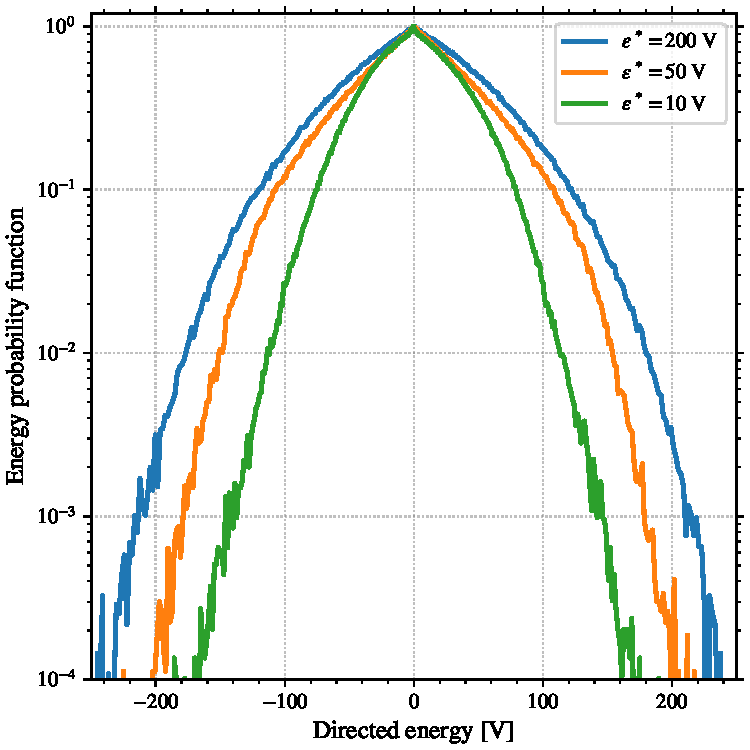
\includegraphics[width=\defaultwidth]{EVDF_Bulk.pdf}
  \caption{Electron velocity distribution function at the center of the simulation, for different values of $\crover$.}
  \label{fig-evdf_epsstar}
\end{figure}

\begin{figure}[hbtp]
  \centering
  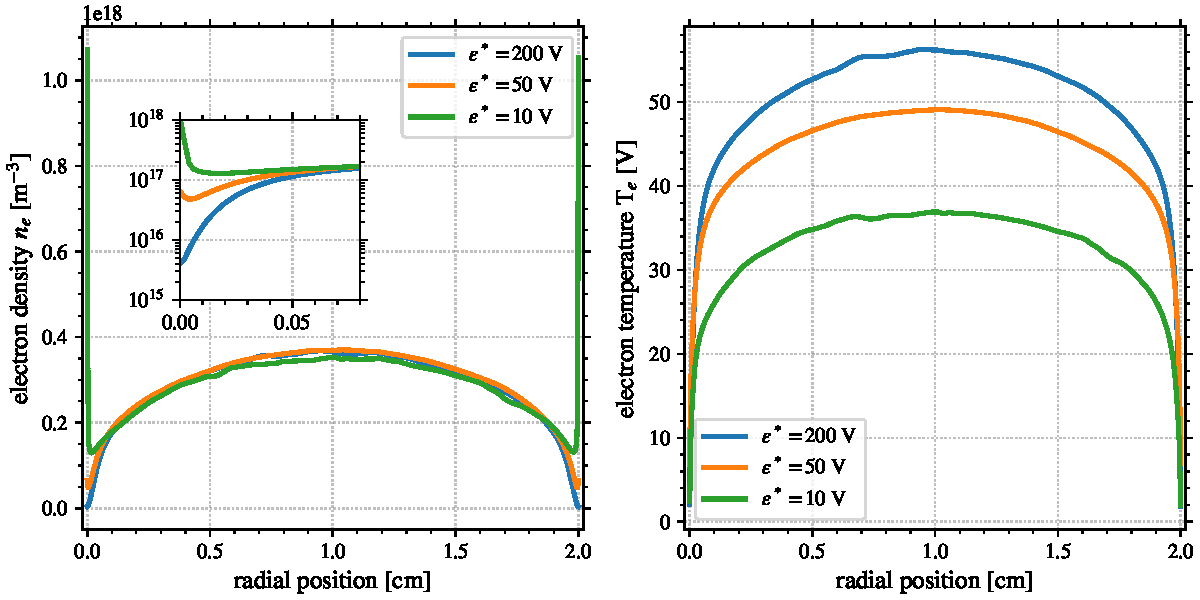
\includegraphics[width=\textwidth]{ne_Te_profiles.pdf}
  \caption{Radial profiles of (left) the electron density and (right) the electron temperature, for different values of $\crover$.}
  \label{fig-radial_profiles_see}
\end{figure}


\begin{figure}[hbtp]
  \centering
  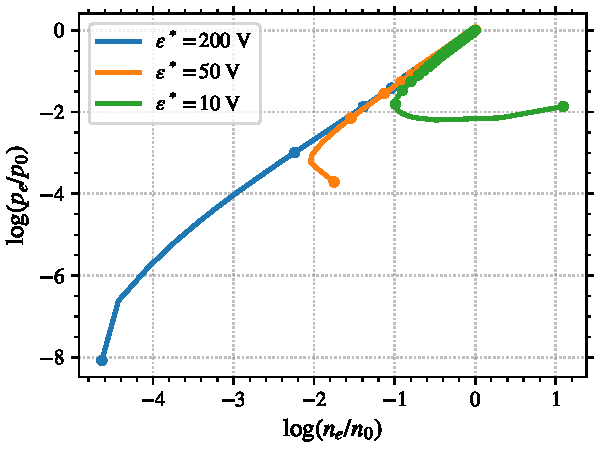
\includegraphics[width=\defaultwidth]{SEE_polytropic_presheath_and_sheath.pdf}
  \caption{electron pressure as a function of the electron density normalized by the center variable, in log scale. Markers are every 10 cells (around 1$\lde$)}
  \label{fig-log_pe-ne}
\end{figure}

\renewcommand\subfigurewidth{3in}

\begin{figure}[hbtp]
  \centering
  \begin{tabular}{c c}
    \subfigure{SEE_polytropic_presheath}{a}{20,20} & 
    \subfigure{SEE_polyfit}{a}{20,20} 
  \end{tabular}
  \caption{Polytropic fit for different values of $\crover$. The sheath (10 cells) are removed from the plots.}
  \label{fig-polyfit_see}
\end{figure}

\FloatBarrier
{\bf Conclusion: $\gamma = 1.35$ in presheath and $\partial{\gamma} / \partial \crover = 0 $}

\paragraph{Hypothesis H1: } Polytropic model until the wall and $\gamma = 1.35$ (might be explained by \cref{{fig-evdf_epsstar}}, and by the fact that we care only on the forward temperature, so not distorted by the secondary electrons).

\paragraph{Hypothesis H2: } From {\bf H1}, and with the 2-$\Te$ hypothesis, we have $\rate = \rate_{\rm Maxw}(\Tew)$, were $\Tew$ can be computed from $Teb$, $\gamma$ and $\dphi$.

\paragraph{Hypothesis H3: } Current equality at the wall : $\Gamma_i + \rate \Gamma_e = \Gamma_e$. This is not a surprising hypothesis.

\section{Sheath model with polytropic electron and SEE}

With {\bf H1, H2} and {\bf H3} we have, as developed in \cref{sec-fluidPIC} with \cref{eq-gi,eq-ge,eq-tew}:
\begin{equation}\label{eq-sheathsee}
  (1 - \rate_{\rm Maxw}(\Tew) )\left[ 1 +\frac{\gamma -1}{\gamma} \frac{ \dphi_0}{ \Te_0}  \right]^{\frac{1}{\gamma - 1}} \sqrt{1 - \frac{\gamma -1}{\gamma}\frac{\dphi_0}{\Te_0}} = \sqrt{\frac{4 \gamma \pi m_e}{m_i}}
\end{equation}
In contrast with \cref{eq-sheath}, now the sheath potential $\Delta \phi$ depends on $\rate$ with depends on $\Te$.
Hence, $\dphi$ is not fully normalized.

\begin{figure}[hbtp]
  \centering
  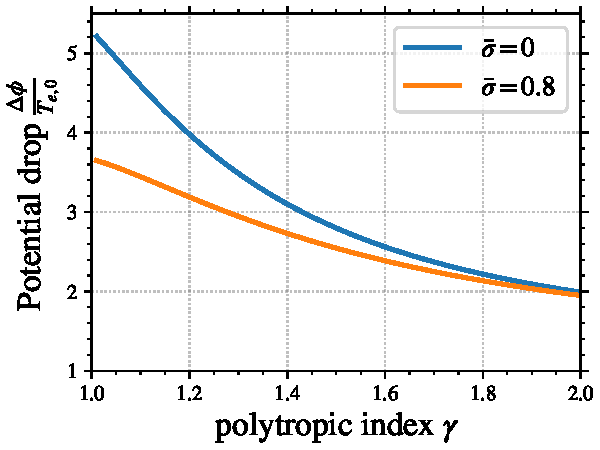
\includegraphics[width=\defaultwidth]{Sheath_drop_with_SEE.pdf}
  \caption{Potential drop $\dphi$ normilized by the bulk electron temperature $\Te_0$ as a function of the polytropic index $\gamma$ for a xenon plasma ($m_i = 131\,\dalton$). The emission rate $\rate$ is fixed for clarity.}
  \label{fig-dphi_see}
\end{figure}

\begin{figure}[hbtp]
  \centering
  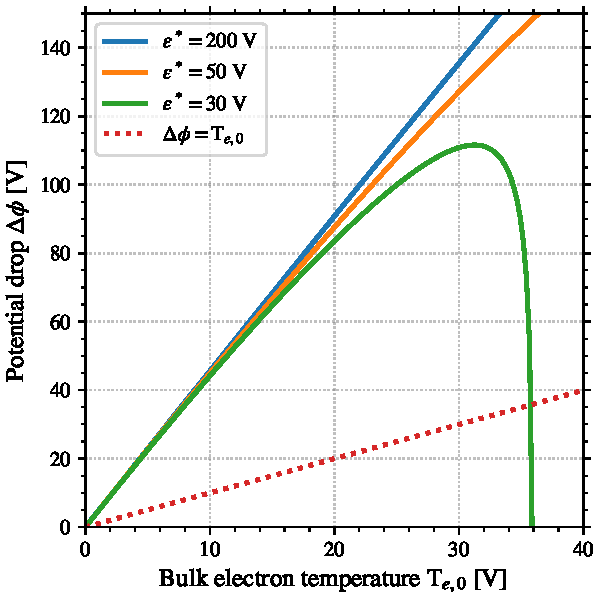
\includegraphics[width=\defaultwidth]{RSO_criteria_polytropic.pdf}
  \caption{ Plasma potential drop to the wall as a function of the electron temperature for different values of the cross-over energy $\crover$ using \cref{eq-sheathsee,eq-seemaxw}. The dashed line is $\dphi=\Te$. Similar to  \cref{fig-dphivsTe} but with polytropic electron of index $\gamma=1.35$}
  \label{fig-rso_crit_see}
\end{figure}

\FloatBarrier

\section{Comparison with PIC simulations} \label{subsec-picandmodel}

\begin{figure}[hbtp]
  \centering
  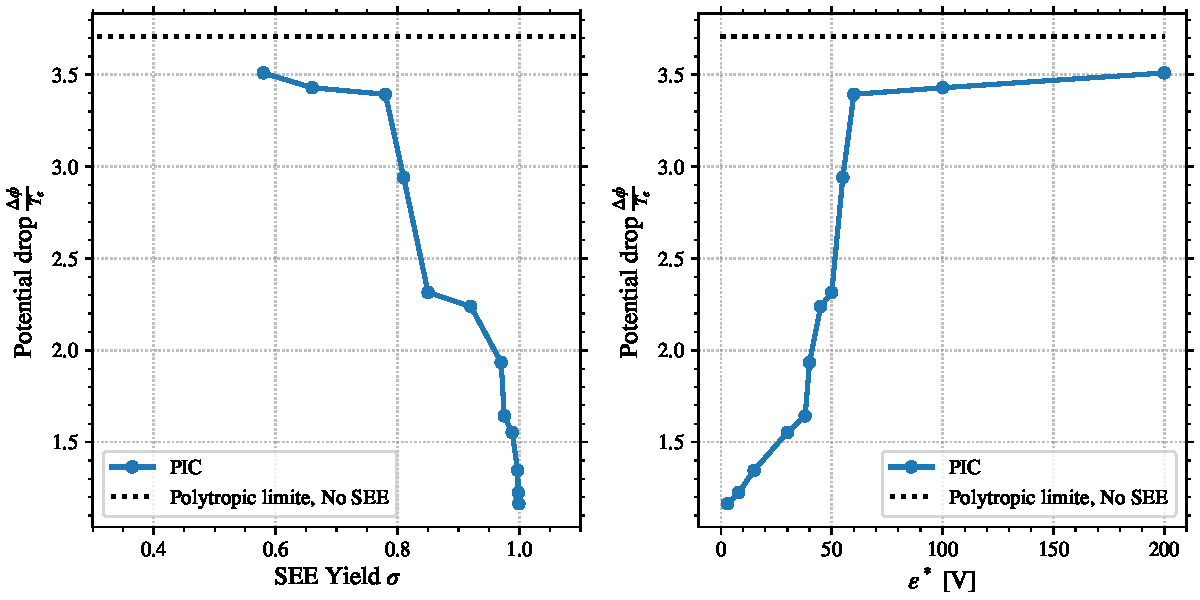
\includegraphics[width=\textwidth]{dphi_polytropic_noSEE}
  \caption{PIC simulation results (with SEE) compared to the polytropic limit without SEE.}
  \label{fig-polytropic_pic_noSEE}
\end{figure}

\begin{figure}[hbtp]
  \centering
  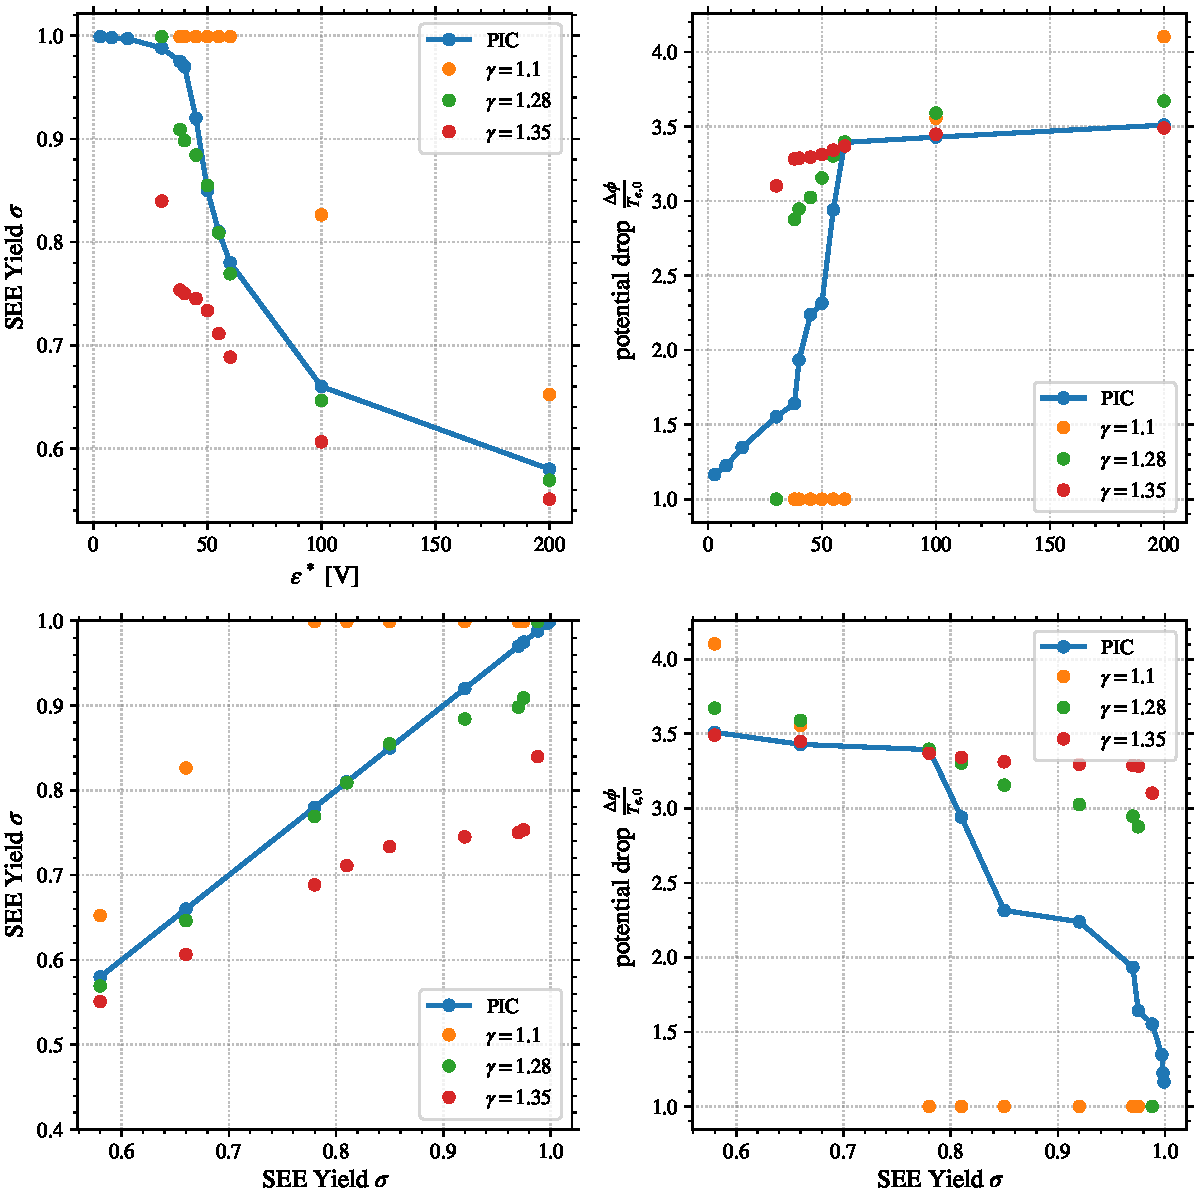
\includegraphics[width=\textwidth]{Summary_polytropic_SEE.pdf}
  \caption{Comparison of the PIC simulation results with the polytropic model with SEE.}
  \label{fig-polytropic_see_summary}
\end{figure}


